\begin{samplecase}
{\bf Residual production cross sections for protons on Fe}\newline
In this sample case, we calculate the residual production cross sections for
protons on ${}^{nat}$Fe for incident energies up to 100 MeV. A calculation for
a natural target is launched, meaning that successive TALYS calculations for
each isotope are performed, after which the results are weighted with the
natural abundance. We restrict ourselves to a calculation with all
nuclear model parameters set to their default values.
The following input file is used:

\VerbatimInput{\samples p-Fe000-rp/org/talys.inp}

The file {\em energies} contains 34 incident energies between 1 and 100 MeV.
Obviously, this sample case can be extended to more incident energies, e.g. up
to 200 MeV, by simply adding numbers to the {\em energies} file. In that case,
we recommend to include more energy bins in the
calculation, (e.g. {\bf bins 80}) to avoid numerical fluctuations, although
this will inevitably take more computer time.
Note that we have enabled the {\bf fileresidual} keyword, so that a separate
cross sections file for each final product is produced.
The results from the files {\em rp027056.tot}, {\em rp027055.tot},
{\em rp025054.tot} and {\em rp025052.tot} are
presented, together with experimental data, in Fig.~\ref{resprod}.
\end{samplecase}
\begin{figure}
\centering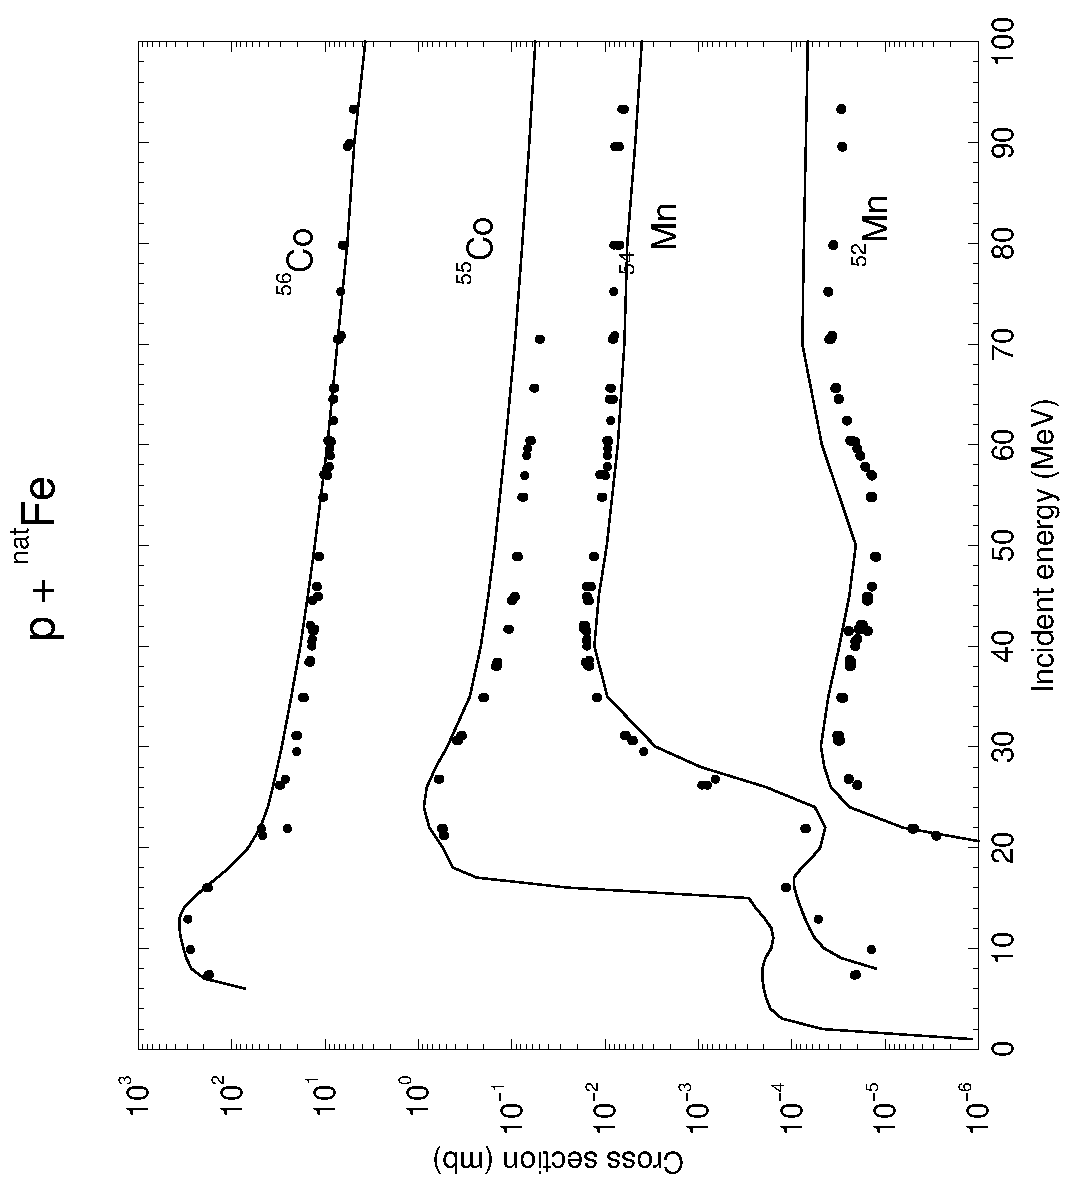
\includegraphics[scale=0.6,angle=270]{feresidual}
\caption{Residual production cross sections for protons incident
on ${}^{nat}$Fe. Experimental data are obtained from \protect\cite{Michel1997}.}
\label{resprod}
\end{figure}

